
\documentclass[11pt]{article}
\usepackage[a4paper,margin=1in]{geometry}
\usepackage{amsmath,amssymb}
\usepackage{graphicx}
\usepackage[dvipsnames]{xcolor}
\usepackage{hyperref}
\usepackage{enumitem}
\usepackage{tabularx}
\usepackage{longtable}
\usepackage{booktabs}
\usepackage[most]{tcolorbox}
\usepackage{titlesec}
\usepackage{xurl}
\usepackage{fancyhdr}
\usepackage{setspace}
\usepackage{tikz}
\usetikzlibrary{positioning,arrows.meta}
\usepackage[T1]{fontenc}
\usepackage{lmodern}
\setlength{\parindent}{0pt}
\setlength{\parskip}{8pt}
\setlength{\headheight}{14pt}
\setstretch{1.12}
\setlist[itemize]{leftmargin=1.5em, nosep}
\setlist[enumerate]{leftmargin=1.5em, nosep}
\providecommand{\tightlist}{\setlength{\itemsep}{0pt}\setlength{\parskip}{0pt}}
\hypersetup{colorlinks=true,linkcolor=MidnightBlue,urlcolor=MidnightBlue}
\pagestyle{fancy}
\raggedbottom
\fancyhf{}
\rhead{\thepage}
\renewcommand{\headrulewidth}{0pt}
\renewcommand{\footrulewidth}{0pt}
\titleformat{\section}{\Large\bfseries\color{MidnightBlue}}{\thesection}{0.6em}{}
\titleformat{\subsection}{\bfseries}{}{0em}{}


\begin{document}

\begin{center}\LARGE\bfseries Block 3 Tutorial -- Reinforcement Learning, Knowledge Graphs, MCP, Multi-Agent Systems, and Coding Agents\end{center}

\begin{center}\large Block 3 Tutorial\end{center}

\begin{tcolorbox}[colback=MidnightBlue!4,colframe=MidnightBlue,title={Session Overview},fonttitle=\bfseries,breakable]
\textbf{Session objective:} Consolidate the whole of Block 3 with longer-form problems that strengthen exam-style reasoning and applied understanding.

\textbf{Timing target (min):} 86

\textbf{Topic anchors:} reinforcement learning; knowledge representation; knowledge graph; mcp; a2a; coding agent; prompt injection

\textbf{Padlet board:} \url{https://padlet.com/qmul/b3-tutorial-uqe9wb7pw5cpxo20}
\end{tcolorbox}

\section*{Exercises}

\begin{tcolorbox}[colback=white,colframe=MidnightBlue,title={Q1 RL Intuition and Credit Assignment},fonttitle=\bfseries,breakable]
\begin{center}
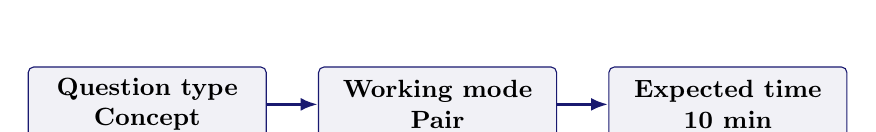
\begin{tikzpicture}[
node distance=0.65cm,
box/.style={draw=MidnightBlue, rounded corners=2pt, minimum height=0.95cm, align=center, font=\small\bfseries, fill=MidnightBlue!6, text width=0.23\linewidth},
arrow/.style={-{Latex[length=2.2mm]}, very thick, MidnightBlue}
]
\node[box] (type) {Question type\\Concept};
\node[box, right=of type] (mode) {Working mode\\Pair};
\node[box, right=of mode] (time) {Expected time\\10 min};
\draw[arrow] (type) -- (mode);
\draw[arrow] (mode) -- (time);
\end{tikzpicture}
\end{center}

{\large\bfseries\color{MidnightBlue} Prompt}\par\medskip
A student says, ``Reinforcement learning is easy because the agent can just wait for the final reward and then know exactly what to do next time.'' Explain why this is not true. Use the idea of delayed reward and credit assignment, and include one everyday example.

{\large\bfseries\color{MidnightBlue} Task details}\par\medskip
\begin{itemize}\item \textbf{Type:} concept
\item \textbf{Mode:} pair
\item \textbf{Time:} 10 min
\item \textbf{Deliverable:} short explanation
\item \textbf{Assessment focus:} connect delayed feedback to credit-assignment difficulty
\item \textbf{Expected length:} 4 bullets\end{itemize}

{\large\bfseries\color{MidnightBlue} How to submit}\par\medskip
Post one pair Padlet comment with four short bullets and one example.

{\large\bfseries\color{MidnightBlue} Discussion in class}\par\medskip
Which part of the action sequence is hardest to assign credit to?

{\large\bfseries\color{MidnightBlue} Why this helps}\par\medskip
Helps with short explanation questions on delayed reward and why RL is hard.

{\large\bfseries\color{MidnightBlue} References}\par\medskip
\begin{itemize}\item Russell \& Norvig (2021) AIMA 4e, Ch.22, pp.789-822
\item Poole \& Mackworth (2023) 3e, Ch.13, pp.583-608\end{itemize}
\end{tcolorbox}

\begin{tcolorbox}[colback=white,colframe=MidnightBlue,title={Q2 RL Update and Interpretation},fonttitle=\bfseries,breakable]
\begin{center}
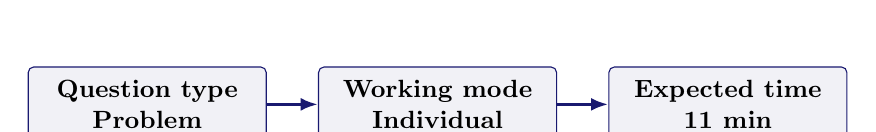
\begin{tikzpicture}[
node distance=0.65cm,
box/.style={draw=MidnightBlue, rounded corners=2pt, minimum height=0.95cm, align=center, font=\small\bfseries, fill=MidnightBlue!6, text width=0.23\linewidth},
arrow/.style={-{Latex[length=2.2mm]}, very thick, MidnightBlue}
]
\node[box] (type) {Question type\\Problem};
\node[box, right=of type] (mode) {Working mode\\Individual};
\node[box, right=of mode] (time) {Expected time\\11 min};
\draw[arrow] (type) -- (mode);
\draw[arrow] (mode) -- (time);
\end{tikzpicture}
\end{center}

{\large\bfseries\color{MidnightBlue} Prompt}\par\medskip
In a delivery task, the agent is in state s4, takes action Wait, receives reward -1, and moves to s5. Suppose Q(s4,Wait)=2.5, max\_a Q(s5,a)=4.0, alpha=0.4, and gamma=0.8. Compute the updated Q-value and explain in one sentence whether the new experience improved or worsened the old estimate.

\begin{tcolorbox}[colback=ForestGreen!5,colframe=ForestGreen,title={Formula reminder},fonttitle=\bfseries,breakable]
\[
Q_{\text{new}}(s,a)=Q(s,a)+\alpha\left[r+\gamma \max_{a'}Q(s',a')-Q(s,a)\right]
\]
\textbf{Use this when the task asks for one update step.}
\end{tcolorbox}

{\large\bfseries\color{MidnightBlue} Task details}\par\medskip
\begin{itemize}\item \textbf{Type:} problem
\item \textbf{Mode:} individual
\item \textbf{Time:} 11 min
\item \textbf{Deliverable:} worked update
\item \textbf{Assessment focus:} compute and interpret one Q-learning update
\item \textbf{Expected length:} 5 lines\end{itemize}

{\large\bfseries\color{MidnightBlue} How to submit}\par\medskip
Post your own Padlet comment with the substitution, the target, the final Q-value, and the interpretation sentence.

{\large\bfseries\color{MidnightBlue} Discussion in class}\par\medskip
Which term in the update carries the long-run estimate?

{\large\bfseries\color{MidnightBlue} Why this helps}\par\medskip
Good practice for RL calculations without reusing the exam numbers.

{\large\bfseries\color{MidnightBlue} References}\par\medskip
\begin{itemize}\item Russell \& Norvig (2021) AIMA 4e, Ch.22, pp.789-822
\item Poole \& Mackworth (2023) 3e, Ch.13, pp.583-608\end{itemize}
\end{tcolorbox}

\begin{tcolorbox}[colback=white,colframe=MidnightBlue,title={Q3 Knowledge Representation with IDs},fonttitle=\bfseries,breakable]
\begin{center}
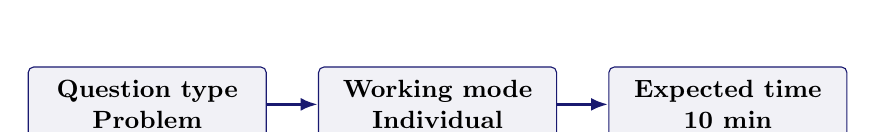
\begin{tikzpicture}[
node distance=0.65cm,
box/.style={draw=MidnightBlue, rounded corners=2pt, minimum height=0.95cm, align=center, font=\small\bfseries, fill=MidnightBlue!6, text width=0.23\linewidth},
arrow/.style={-{Latex[length=2.2mm]}, very thick, MidnightBlue}
]
\node[box] (type) {Question type\\Problem};
\node[box, right=of type] (mode) {Working mode\\Individual};
\node[box, right=of mode] (time) {Expected time\\10 min};
\draw[arrow] (type) -- (mode);
\draw[arrow] (mode) -- (time);
\end{tikzpicture}
\end{center}

{\large\bfseries\color{MidnightBlue} Prompt}\par\medskip
A campus assistant must answer: Which room hosts EBU6505 today, who teaches it, and how can a student contact the lecturer? Write seven triples using stable IDs, and make sure one of your triples stores a contact channel correctly.

{\large\bfseries\color{MidnightBlue} Task details}\par\medskip
\begin{itemize}\item \textbf{Type:} problem
\item \textbf{Mode:} individual
\item \textbf{Time:} 10 min
\item \textbf{Deliverable:} triple set
\item \textbf{Assessment focus:} write stable triples with entities, relations, and attributes
\item \textbf{Expected length:} 7 triples\end{itemize}

{\large\bfseries\color{MidnightBlue} How to submit}\par\medskip
Post your own Padlet comment with seven triples and clear IDs.

{\large\bfseries\color{MidnightBlue} Discussion in class}\par\medskip
Which information is better stored as an attribute than as a linked entity?

{\large\bfseries\color{MidnightBlue} Why this helps}\par\medskip
Consolidates triple design and ID choices.

{\large\bfseries\color{MidnightBlue} References}\par\medskip
\begin{itemize}\item Russell \& Norvig (2021) AIMA 4e, Ch.10, pp.314-343
\item Poole \& Mackworth (2023) 3e, Ch.16, pp.701-730\end{itemize}
\end{tcolorbox}

\begin{tcolorbox}[colback=white,colframe=MidnightBlue,title={Q4 Graph Path, Provenance, and Context},fonttitle=\bfseries,breakable]
\begin{center}
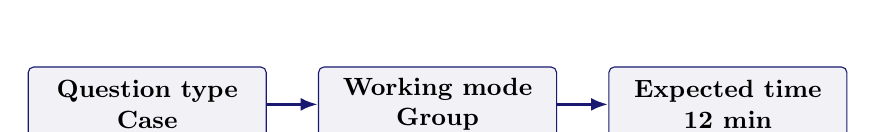
\begin{tikzpicture}[
node distance=0.65cm,
box/.style={draw=MidnightBlue, rounded corners=2pt, minimum height=0.95cm, align=center, font=\small\bfseries, fill=MidnightBlue!6, text width=0.23\linewidth},
arrow/.style={-{Latex[length=2.2mm]}, very thick, MidnightBlue}
]
\node[box] (type) {Question type\\Case};
\node[box, right=of type] (mode) {Working mode\\Group};
\node[box, right=of mode] (time) {Expected time\\12 min};
\draw[arrow] (type) -- (mode);
\draw[arrow] (mode) -- (time);
\end{tikzpicture}
\end{center}

{\large\bfseries\color{MidnightBlue} Prompt}\par\medskip
Your graph says Module\_EBU6505 taughtBy Dr\_Riasat\_Islam, Dr\_Riasat\_Islam officeRoom TB\_3\_335, and a newer notice says officeRoom temporaryRoom QM\_4\_201 for this week only. Explain how the assistant should answer a student asking ``Where can I find the lecturer today?'' Include the graph path, the role of provenance, and what should go into the final context packet.

{\large\bfseries\color{MidnightBlue} Task details}\par\medskip
\begin{itemize}\item \textbf{Type:} case
\item \textbf{Mode:} group
\item \textbf{Time:} 12 min
\item \textbf{Deliverable:} reasoning path with trust note
\item \textbf{Assessment focus:} use a graph path and explain what provenance changes
\item \textbf{Expected length:} 1 path + 2 trust notes\end{itemize}

{\large\bfseries\color{MidnightBlue} How to submit}\par\medskip
Post one group Padlet comment with the path, the answer policy, and two notes on provenance or evidence selection.

{\large\bfseries\color{MidnightBlue} Discussion in class}\par\medskip
Why is the newer fact not enough on its own without provenance?

{\large\bfseries\color{MidnightBlue} Why this helps}\par\medskip
Helps with graph reasoning and evidence-quality questions.

{\large\bfseries\color{MidnightBlue} References}\par\medskip
\begin{itemize}\item Russell \& Norvig (2021) AIMA 4e, Ch.10, pp.314-343
\item Poole \& Mackworth (2023) 3e, Ch.16-17, pp.701-766\end{itemize}
\end{tcolorbox}

\begin{tcolorbox}[colback=white,colframe=MidnightBlue,title={Q5 MCP Workflow Check},fonttitle=\bfseries,breakable]
\begin{center}
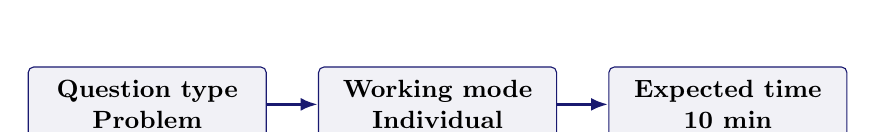
\begin{tikzpicture}[
node distance=0.65cm,
box/.style={draw=MidnightBlue, rounded corners=2pt, minimum height=0.95cm, align=center, font=\small\bfseries, fill=MidnightBlue!6, text width=0.23\linewidth},
arrow/.style={-{Latex[length=2.2mm]}, very thick, MidnightBlue}
]
\node[box] (type) {Question type\\Problem};
\node[box, right=of type] (mode) {Working mode\\Individual};
\node[box, right=of mode] (time) {Expected time\\10 min};
\draw[arrow] (type) -- (mode);
\draw[arrow] (mode) -- (time);
\end{tikzpicture}
\end{center}

{\large\bfseries\color{MidnightBlue} Prompt}\par\medskip
A student proposes this MCP workflow: tool call -\textgreater{} user intent parse -\textgreater{} response synthesis -\textgreater{} capability discovery -\textgreater{} audit log -\textgreater{} evidence return. Rewrite it into a sensible order and explain two mistakes in the original version.

{\large\bfseries\color{MidnightBlue} Task details}\par\medskip
\begin{itemize}\item \textbf{Type:} problem
\item \textbf{Mode:} individual
\item \textbf{Time:} 10 min
\item \textbf{Deliverable:} corrected workflow
\item \textbf{Assessment focus:} understand the parts and ordering of an MCP interaction
\item \textbf{Expected length:} 6 steps + 2 fixes\end{itemize}

{\large\bfseries\color{MidnightBlue} How to submit}\par\medskip
Post your own Padlet comment with the corrected order and two explained mistakes.

{\large\bfseries\color{MidnightBlue} Discussion in class}\par\medskip
Which mistake is most dangerous for safety?

{\large\bfseries\color{MidnightBlue} Why this helps}\par\medskip
Consolidates MCP flow understanding in a fresh scenario.

{\large\bfseries\color{MidnightBlue} References}\par\medskip
\begin{itemize}\item https://modelcontextprotocol.io/specification/
\item Russell \& Norvig (2021) AIMA 4e, Ch.10, pp.314-343\end{itemize}
\end{tcolorbox}

\begin{tcolorbox}[colback=white,colframe=MidnightBlue,title={Q6 Multi-Agent and A2A Design},fonttitle=\bfseries,breakable]
\begin{center}
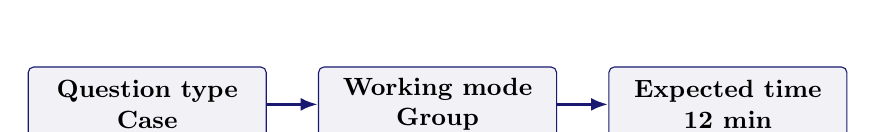
\begin{tikzpicture}[
node distance=0.65cm,
box/.style={draw=MidnightBlue, rounded corners=2pt, minimum height=0.95cm, align=center, font=\small\bfseries, fill=MidnightBlue!6, text width=0.23\linewidth},
arrow/.style={-{Latex[length=2.2mm]}, very thick, MidnightBlue}
]
\node[box] (type) {Question type\\Case};
\node[box, right=of type] (mode) {Working mode\\Group};
\node[box, right=of mode] (time) {Expected time\\12 min};
\draw[arrow] (type) -- (mode);
\draw[arrow] (mode) -- (time);
\end{tikzpicture}
\end{center}

{\large\bfseries\color{MidnightBlue} Prompt}\par\medskip
Design a student-support workflow with a coordinator agent, retrieval agent, policy-check agent, and message-draft agent. Include one A2A handoff to an external scholarship-information agent and one trust check before the answer is accepted.

{\large\bfseries\color{MidnightBlue} Task details}\par\medskip
\begin{itemize}\item \textbf{Type:} case
\item \textbf{Mode:} group
\item \textbf{Time:} 12 min
\item \textbf{Deliverable:} orchestration sketch
\item \textbf{Assessment focus:} design a trustworthy multi-agent workflow with one A2A handoff
\item \textbf{Expected length:} 5 bullets\end{itemize}

{\large\bfseries\color{MidnightBlue} How to submit}\par\medskip
Post one group Padlet comment with the role order, the handoff point, and the trust check.

{\large\bfseries\color{MidnightBlue} Discussion in class}\par\medskip
Which agent should never be allowed to act without evidence from another component?

{\large\bfseries\color{MidnightBlue} Why this helps}\par\medskip
Builds confidence for architecture and handoff questions in a new scenario.

{\large\bfseries\color{MidnightBlue} References}\par\medskip
\begin{itemize}\item https://a2a-protocol.org/dev/
\item doi:10.1016/j.cosrev.2026.100902\end{itemize}
\end{tcolorbox}

\begin{tcolorbox}[colback=white,colframe=MidnightBlue,title={Q7 Coding-Agent Safety Review},fonttitle=\bfseries,breakable]
\begin{center}
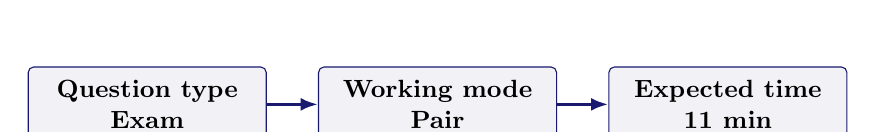
\begin{tikzpicture}[
node distance=0.65cm,
box/.style={draw=MidnightBlue, rounded corners=2pt, minimum height=0.95cm, align=center, font=\small\bfseries, fill=MidnightBlue!6, text width=0.23\linewidth},
arrow/.style={-{Latex[length=2.2mm]}, very thick, MidnightBlue}
]
\node[box] (type) {Question type\\Exam};
\node[box, right=of type] (mode) {Working mode\\Pair};
\node[box, right=of mode] (time) {Expected time\\11 min};
\draw[arrow] (type) -- (mode);
\draw[arrow] (mode) -- (time);
\end{tikzpicture}
\end{center}

{\large\bfseries\color{MidnightBlue} Prompt}\par\medskip
A coding agent is asked to modify a grading script in a live course repository. Explain what context it must collect first, one risk from repository text, one risk from tool use, and one human checkpoint that should not be skipped.

{\large\bfseries\color{MidnightBlue} Task details}\par\medskip
\begin{itemize}\item \textbf{Type:} exam
\item \textbf{Mode:} pair
\item \textbf{Time:} 11 min
\item \textbf{Deliverable:} risk-focused response
\item \textbf{Assessment focus:} explain a safe coding-agent workflow with controls
\item \textbf{Expected length:} 180-220 words\end{itemize}

{\large\bfseries\color{MidnightBlue} How to submit}\par\medskip
Post one pair Padlet comment with a clear structure covering context, two risks, and the checkpoint.

{\large\bfseries\color{MidnightBlue} Discussion in class}\par\medskip
Which repository risk is easiest for students to underestimate?

{\large\bfseries\color{MidnightBlue} Why this helps}\par\medskip
Consolidates coding-agent governance and safety without duplicating the exam pull-request question.

{\large\bfseries\color{MidnightBlue} References}\par\medskip
\begin{itemize}\item https://openai.com/codex/
\item https://docs.anthropic.com/en/docs/claude-code/overview
\item https://genai.owasp.org/resource/agentic-ai-threats-and-mitigations/\end{itemize}
\end{tcolorbox}

\begin{tcolorbox}[colback=white,colframe=MidnightBlue,title={Q8 Stretch Synthesis},fonttitle=\bfseries,breakable]
\begin{center}
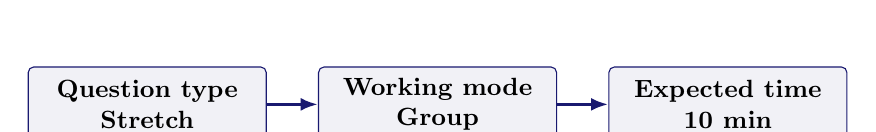
\begin{tikzpicture}[
node distance=0.65cm,
box/.style={draw=MidnightBlue, rounded corners=2pt, minimum height=0.95cm, align=center, font=\small\bfseries, fill=MidnightBlue!6, text width=0.23\linewidth},
arrow/.style={-{Latex[length=2.2mm]}, very thick, MidnightBlue}
]
\node[box] (type) {Question type\\Stretch};
\node[box, right=of type] (mode) {Working mode\\Group};
\node[box, right=of mode] (time) {Expected time\\10 min};
\draw[arrow] (type) -- (mode);
\draw[arrow] (mode) -- (time);
\end{tikzpicture}
\end{center}

{\large\bfseries\color{MidnightBlue} Prompt}\par\medskip
Propose a small university assistant architecture that uses structured knowledge, one graph-backed retrieval step, one MCP tool interaction, and one safety rule for any coding or tool-using agent component.

{\large\bfseries\color{MidnightBlue} Task details}\par\medskip
\begin{itemize}\item \textbf{Type:} stretch
\item \textbf{Mode:} group
\item \textbf{Time:} 10 min
\item \textbf{Deliverable:} short architecture proposal
\item \textbf{Assessment focus:} combine Block 3 ideas into one system design
\item \textbf{Expected length:} 6 bullets\end{itemize}

{\large\bfseries\color{MidnightBlue} How to submit}\par\medskip
Post one group Padlet comment with six bullets describing the architecture.

{\large\bfseries\color{MidnightBlue} Discussion in class}\par\medskip
Which Block 3 idea gives the biggest practical benefit in your design?

{\large\bfseries\color{MidnightBlue} Why this helps}\par\medskip
Helps students synthesise Block 3 without mirroring any single exam question.

{\large\bfseries\color{MidnightBlue} References}\par\medskip
\begin{itemize}\item Russell \& Norvig (2021) AIMA 4e, Ch.10, pp.314-343 and Ch.22, pp.789-822
\item Poole \& Mackworth (2023) 3e, Ch.13, pp.583-608 and Ch.16-17, pp.701-766
\item https://modelcontextprotocol.io/specification/\end{itemize}
\end{tcolorbox}

\section*{Submission Instructions}

Use the seeded Padlet posts for Q1--Q8. Q2, Q3, and Q5 are individual. Q1 and Q7 are pair tasks. Q4, Q6, and Q8 should be one joint group comment. Start each comment with your names or group label.

\section*{Whole-Class Debrief Prompts}

\begin{itemize}
\tightlist
\item
  Which Block 3 idea still feels the least intuitive?
\item
  Which exercise was closest to ``exam thinking'' without being an exam copy?
\item
  Where do safety and structure interact most strongly across the whole block?
\end{itemize}

\section*{Exam Transfer Note (Day-Level)}

This tutorial consolidates RL, structured knowledge, graphs, MCP, A2A, and coding-agent safety in a way that supports exam preparation across fresh scenarios.

\end{document}
